\documentclass[a4paper]{article}
\usepackage[spanish]{babel}
\usepackage[utf8]{inputenc}
\usepackage{graphicx}
\usepackage{biblatex}
\usepackage{enumerate}
\usepackage{csquotes}
\usepackage{braket}
\usepackage{amsmath}

\title{Spiking neurons}
\begin{document}
\maketitle
\section{Estabilidad}
Las ecuaciones que describen al sistema son:
$$\dot{r}=\frac{\Delta}{\pi}+2rv$$
$$\dot{v}=v^2+\bar{\eta}+Jr-\pi^2 r^2 + I(t)$$
Para saber las nulclinas tomamos $\dot{r}=0$ y $\dot{v} = 0$.
$$\frac{\Delta}{\pi}+2rv=0 \Rightarrow r = -\frac{\Delta}{2 \pi v}$$
$$v^2+\bar{\eta}+Jr-\pi^2 r^2 + I(t) = 0$$
Los puntos de estabilidad los obtenemos con los puntos de corte de estas dos funciones.
El campo vectorial lo obtenemos dando valores a r y a v en el el sistema:
$$\dot{r}=\frac{\Delta}{\pi}+2rv$$
$$\dot{v}=v^2+\bar{\eta}+Jr-\pi^2 r^2 + I(t)$$
siendo $\dot{r}$ la componente en x de cada vector y $\dot{v}$ la componente en y. 
Para saber el tipo de estabilidad en cada punto tomamos las funciones:
$$f(r,v) = \frac{\Delta}{\pi}+2rv$$
$$g(r,v) = v^2+\bar{\eta}+Jr-\pi^2 r^2 + I(t)$$
$$
\begin{pmatrix} \dot{r} \\ \dot{v} \end{pmatrix} = 
\begin{pmatrix}
\frac{\partial f}{\partial r} & \frac{\partial f}{\partial v} \\
\frac{\partial g}{\partial r} & \frac{\partial g}{\partial v}
\end{pmatrix}
\begin{pmatrix} r \\ v \end{pmatrix}
$$
$$
\begin{pmatrix} \dot{r} \\ \dot{v} \end{pmatrix} = 
\begin{pmatrix}
2v & 2r \\
J - 2\pi^2 r & 2v
\end{pmatrix}
\begin{pmatrix} r \\ v \end{pmatrix}
$$
$$Tr = 4v$$
$$det = 4v^2 - 2rJ + 4\pi^2 r^2$$
\section{Pasos a seguir}
día 12/02/2020 \\
El programa funciona igual que en el paper. (PONER ALGUNAS IMÁGENES). El próximo paso a seguir es comprobar el diagrama de fases.\\

día 13/02/2020\\
Sabemos que $r = nºspiking Neurons/(N*dt)$\\
Para $J = 15$ tenemos el siguiente diagrama:\\
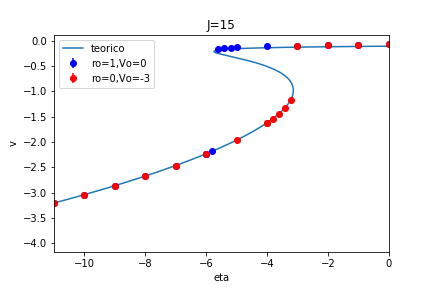
\includegraphics[scale=0.7]{v_vs_eta_J15.png}\\
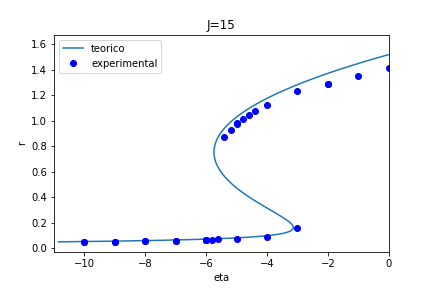
\includegraphics[scale=0.7]{r_vs_eta_J15.png}\\
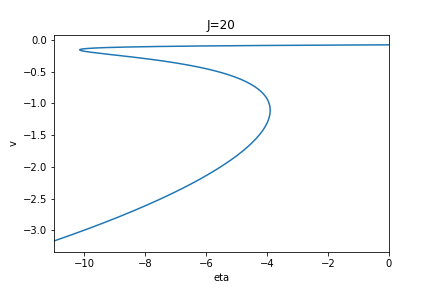
\includegraphics[scale=0.7]{v_vs_eta_J20.png}\\
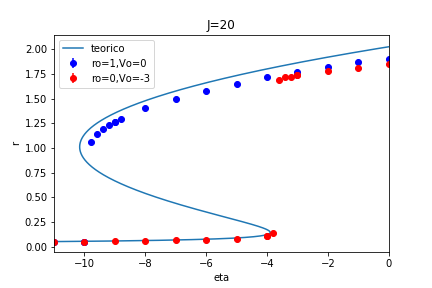
\includegraphics[scale=0.7]{r_vs_eta_J20.png}\\
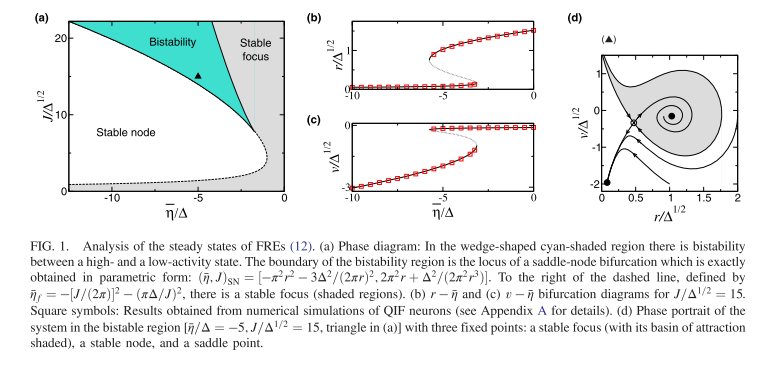
\includegraphics[scale=0.4]{diagramaspaper.png}\\
Para demostrar la biestabilidad primero vamos a la primera zona de estabilidad en $ \bar{\eta} = -5$:
$r\simeq 1$ y $ v\simeq 0$
para obtener  $r = 1$
$$nºspikingNeurons/Ndt = 1$$
con $N = 10^4$ y $dt = 10^{-4}$
entonces en cada intervalo temporal
$$nºspikingNeurons = 1$$
Esto lo mantenemos durante 5s y luego dejamos 10s al sistema para relajarse.
\end{document}
